\documentclass[serif,mathserif,final]{beamer}
\mode<presentation>{\usetheme{Lankton}}
\usepackage{amsmath,amsfonts,amssymb,pxfonts,eulervm,xspace}
\usepackage{graphicx}
\graphicspath{{./fig/}}
\usepackage[orientation=landscape,size=custom,width=40,height=30,scale=.6,debug]{beamerposter}
\setbeamertemplate{caption}[numbered]

%-- Header and footer information ----------------------------------
\newcommand{\footleft}{https://github.com/hsavoy/cs267FinalProject}
\newcommand{\footright}{longva@berkeley.edu \quad frystacka@berkeley.edu}
\title{Parallel Empirical Variogram Calculation for Large Datasets}
\author{Andreas Borgen Longva \quad Heather Savoy}
\institute{University of California, Berkeley}
%-------------------------------------------------------------------


%-- Main Document --------------------------------------------------
\begin{document}
\begin{frame}{}
  \begin{columns}[t]

    %-- Column 1 ---------------------------------------------------
    \begin{column}{0.32\linewidth}

      %-- Block 1-1
      \begin{block}{Motivation}
   
	 \begin{itemize}
	 	\item Spatial heterogeneity in an aquifer significantly affects contaminant transport in groundwater
		\item A way is needed to incorporate the uncertainty about the aquifer in groundwater modeling (geostatistics!)
         
         \begin{figure}[htbp]
            \centering
            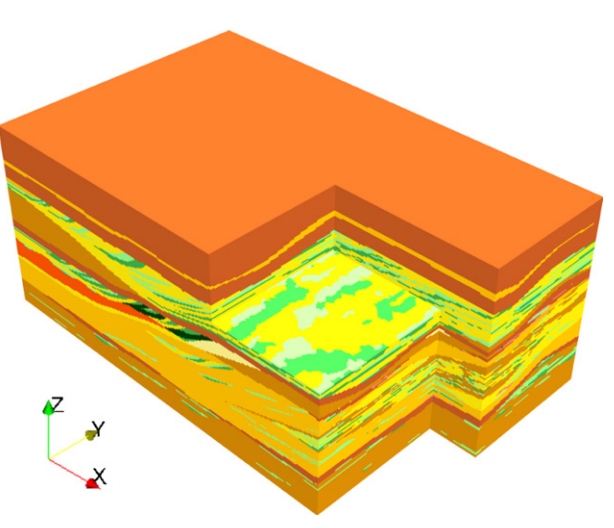
\includegraphics[height=7cm]{herten.png} % requires the graphicx package
            \caption{Large aquifer data set : $n=8.96\times 10^6$ \cite{Comunian2011a}}
            \label{fig:example}
         \end{figure}
         
         \item The data set above can be used to study realistic geologic patterns, but it is too big for serial geostatistical algorithms
         \item \textbf{Goal}: Implement parallel algorithm to analyze the data set in reasonable time
          \end{itemize}
      \end{block}

      %-- Block 1-2
      \begin{block}{Geostatistics}
      Variograms describe how properties are correlated over space:
        \begin{equation*}
		\hat{\gamma}(h)=\frac{1}{2|N(h)|}\sum_{(i,j)\in N(h)} |z_i-z_j|^2
	\end{equation*}
	where $h$ is distance between points $i$ and $j$, which have value $z_i$ and $z_j$. The algorithm is $O(n^2)$ and involves all-to-all communications.
	
      \end{block}
  

    \end{column}%1

    %-- Column 2 ---------------------------------------------------
    \begin{column}{0.32\linewidth}

      %-- Block 2-1
      \begin{block}{Implementation}
      \center{Work is divided for pairs, not points}
	
	~
	
      \begin{flushleft} Modified algorithm from \cite{Koanantakool}:
        \begin{enumerate}
          \item $p$ processors divided into teams of size $p/c$, where $c$ is an integer up to how many copies of points that can fit in memory
          \item points distributed evenly to team leaders
          \item maximum distance between points determined with reduce sum
          \item team leaders broadcast local points to team members
          \item local points copied into an exchange buffer
          \item shift exchange buffer by rank in team across teams
          \item loop $p/c^2$ times: shift exchange buffer by c across teams, compute squared differences and store in local buffer
          \item reduce sum for global $\hat{\gamma}(h)$ and $N(h)$
          \item divide $\hat{\gamma}(h)$ by $N(h)$
        \end{enumerate}
        \end{flushleft}
      \end{block}

    \end{column}%2

    %-- Column 3 ---------------------------------------------------
    \begin{column}{0.32\linewidth}

      %-- Block 3-1
      \begin{block}{Timing Results}
        \begin{figure}[htbp]
            \centering
            \includegraphics[height=10cm]{comm_c1_scaling.png} % requires the graphicx package
            %\caption{}
            \label{fig:plot}
         \end{figure}
      \end{block}

      %-- Block 3-2
      \begin{block}{Conclusion and Outlook}
        \begin{itemize}
         \item Near-perfect scaling for large n
         \item 
         \item Effect of c:
         \item Empirical variogram for data set in Figure \ref{fig:example} can be obtained in ... with ? processors
        \end{itemize}
      \end{block}

      %-- Block 3-3
      \begin{block}{References}
        \bibliographystyle{plain}
	{\footnotesize
	\bibliography{ref}}
      \end{block}

    \end{column}%3

  \end{columns}
\end{frame}
\end{document}
